\documentclass[a4paper]{report}

\usepackage[12pt]{extsizes} % Нестандартный размер кегля
\usepackage[russian]{babel} % Правильные переносы слов в конце строки
\usepackage[utf8]{inputenc} % Кодировка файла -- utf8
\usepackage{amsmath, amssymb} % Математические символы
\usepackage{fancyhdr}
\usepackage[usenames]{color}
\usepackage{colortbl}
\usepackage{lastpage}
\usepackage{enumitem} % Расширенные перечисления
\usepackage{titlesec}
\usepackage{titletoc}
\usepackage{csquotes} % Оформление цитат
\usepackage[document]{ragged2e}
\usepackage{graphicx}
\graphicspath{{pics/}} % Узакываем путь до картинок
\usepackage{subcaption}
\usepackage{multirow}
\usepackage{wrapfig}
\usepackage{xcolor}
\usepackage{hyperref}


\voffset=-20mm
\textheight=250mm
\hoffset=-20mm
\textwidth=180mm
\headsep=12pt
\footskip=40pt

\pagestyle{empty}
\cfoot{\large \thepage \ of \pageref*{LastPage}}
\renewcommand{\headrulewidth}{0pt}
\renewcommand{\footrulewidth}{0.4pt}
\fancypagestyle{fchapter}{
  \lhead{}
  \rhead{}
  \cfoot{\large \thepage \ of \pageref*{LastPage}}
  \renewcommand{\headrulewidth}{0pt}
  \renewcommand{\footrulewidth}{0.4pt}
}
\fancypagestyle{fstyle}{
  \headheight=30pt
  \footskip=30pt
  \lhead{\Huge \bf ML}
  \rhead{\large \leftmark}
  \renewcommand{\headrulewidth}{0.4pt}
  \renewcommand{\footrulewidth}{0.4pt}
}
\pagestyle{fstyle}

\renewcommand{\section}[1]{
  \refstepcounter{section}
  \vspace*{2em}
  \addcontentsline{toc}{section}{#1}
  {\bf\Large #1}
  \vspace*{1em}
}
\titleformat{\chapter}[hang]
  {\Huge}{Lecture \thechapter:}{1em}
  {\thispagestyle{fchapter}}
\renewcommand{\chaptermark}[1]{
  \markboth{Lecture~\thechapter: #1}{}
}

\addto\captionsrussian{
  \renewcommand{\contentsname}{Contents}
}
\titlecontents{chapter}[0em]{\vskip 0.5ex}{\bf\large}{\bf\large}{}

\definecolor{sapphireblue}{rgb}{0.06,0.32,0.73}
\hypersetup{
    colorlinks,
    linkcolor=sapphireblue,
    urlcolor=sapphireblue,
}


\begin{document}

\begingroup
  \hypersetup{linkcolor=black}
  \tableofcontents
\endgroup

\chapter{kNN}

{\sf Nothing to see here.}


<...>

\chapter{Clustering}

{\sf Nothing to see here.}


<...>

\chapter{Desicion Trees}

{\sf Nothing to see here.}


<...>

\chapter{Ensemble Methods}

{\sf Ensemble method is just uniting the outputs of several classifiers into one. So let's say we have the three clasifiers (in that case you already familiar with KNN and Desicion Trees, you will be familiar with Support Vector Machines in a couple of lectures). We have three clasifiers and they have different outputs for different class in your space. You can merge those predictions into the one and have a unified answer. The simple way to do it is called voting.}

\section{Voting}

 The voting can be hard or soft; the first one when we just count the number of votes, for example, if I have five trees and most of them get class A as an answer, so my answer will be A class. If we have the even number of trees and the half of them say <<Сlass A is the answer>> and others say <<Class B is the answer>>, we have to deal with it by taking into account where they are not, you want the Higher Presicion or Higher Recall or just piking the classes in alphabetical order (the last one is the way it is done in Scikit-learn, so if you use this package, be aware of that). You can work around it by having an odd number of classifiers. Soft voting takes into account how sure the classifier in this desicion. For example, two classifiers get pair (0.1, 0.9) as an answer (0.1 is the probability of class A, 0.9 is the probability of class B) and three classifiers says <<Not sure>> (pair (0.51, 0.49)). The hard voting will give us class A as an answer (because last three get class A), however you see that that three trees don't actually give as an answer, because (0.51, 0.49) is so close to the neutral answer (0.5, 0.5). In soft voting you either end up the points for each class of the probablities, or you multiply, or you add, and then you can take an answer.

\section{Random Forest}

The one of the best algotithms which utilizes the voting system is called Random Forest, and just from the name of own you can guess that the classifiers are trees, but what makes it random? It is a sampling strategy. We only have our dataset, we don't have all the data points but let's simulate sampling from the general data by sampling from the dataset. And now let's build a tree for each sample and this will helps us find a noise. [Забегая вперед: мы строим каждое дерево не на всем объеме данных, а на какой-то его части. Эту часть мы будем выбирать исходя из некоторых весов точек. Сами веса при этом меняются после каждого построения дерева. Еще можно брать все точки, а веса как-то учитывать при построении деревьев.]\\
The greatest thing about random forest is the more trees you have the better random forest is: there is no owerfitting over the number of trees. So there are sampling strategies we mostly use the combination of bagging and random subspaces but let's just go through all of them.

\subsubsection*{Pasting}

Pasting is a simple sampling: let's take out of $N$ points $K$ random with no repeats.

\subsubsection*{Bagging (bootstrap agregating)}

The bagging (also bootstrap agregating) is a statistical term means the situation when you take the dataset of a sample with the same size but with repeats. Let's say we have the dataset with some features and two classes of the points from the dataset. Also we have weights for all points. That means that when we end up the error we multiply an error of every point by the weight of that point. The thing we gonna do the most today is manipulate that weight. \\
Let's imagine we want to take the points with repeats. If the sampling weights are the same, you can just take a random point. If the sampling weights are different and you want to sample with those weights, you can do the thing we did when we thought about how to sample in k-means$++$ algorithm. <...> \\
So you can use some weights in your classifier: when you build a tree, for example, you use the Gini formula ($\sum_{y\in Y}\frac{1}{|X|}\cdot|x: y(x) =y|\cdot|x: y(x) \ne y|$) but instead of counting the number of points you can add up their weights. There are different strategies for sampling; you can pick points according to the probability or you can just use this probability as your weights in your impurity calculation. Also instead of taking random samples of $N$ we can just assign a random numbers as weights and the best thing approximates bootstraping is a Poisson distribution so you can just select random numbers of the Poisson distribution and then use those numbers as weights in your impurity calculation.

\subsubsection*{Random subspaces}

The random subspaces is a way to try to randomize it and do a good work around noise anymore. We don't take random samples but rather we take random features so let's just use some subspace of features and random patches is both. So we use both random sample and random feature. Now you can natively calculate what is called feature importanse: if you want to now how important is your feature to the algorithm, you can build many trees and you can just calculate the number of trees that feature participates in. 

\subsubsection*{Extremely randomized trees}

Extremely randomized trees: instead of going over all the thresholds, over all the features, you can just say <<Ok, let's pick a hundred random thresholds and then pick the best>>. It doesn't work by itself, so if you want to construct one tree you will construct a really bad tree. However if you want to construct a forest, that not a bad idea. You can construct a good forest with extremly randomized trees.\\
{\it <Some talk about how random forests are good.>}\\
{\it <A meme slide about bootstraps and Munchausen...>}

\section{Boosting Algorithms}

Random forests constructs each tree basicaly independently, which is good because we can parellelize it. However, let's say we construct our first tree and it gives us a realy good answer with only a couple of problem points. In that case we would not want the next tree to be random, we would rather want the next tree to take into account the results of the first tree. The algorithms what do that are called Boosting Algorithms. It is important to know that we don't actually need to build a deep trees. So in the random forest we prefer to use trees with depth 5 or 6, and in adaptive boosting we use stumps (trees with only two leaves). In gradient boosting we use trees with depth 3 or 4. 

\subsubsection*{Adaptive Boosting}

So we have our dataset and the first thing we do is we construct the first classifier that gives us the answer. <...>\\
At the first step we do the weights is uniform, so every point has the weight $D_1(i)=\frac{1}{N}$. Then you build a tree to minimize error $E_t = \sum_{i=1}^N D_t(i) \cdot E(h_t(x_i), y_i)$ [в простом варианте $E(h_t(x),y) = 1$, если не угадали класс и $0$, если угадали]. So you just select the best threshold of all features and then you assign the weight $\alpha_t=\frac{1}{2}\ln(\frac{1-E_t}{E_t})$ for that tree. {\it <A little description of this function and how it helps us>} Now you need to recalculate weights:
$$\begin{cases}
D_{t+1}(i) = D_t(i)e^{\alpha_t}&\text{for incorrectly classified points,}\\
D_{t+1}(i)=D_t(i)e^{-\alpha_t}&\text{for correctly classified points.}
\end{cases}$$
Now you have the new sampling weights and you need to repeat the process, creating a new trees. You should stop if you don't have any improvement in your impurity, when you take into account the weights. The final hypothesys suggests the some number (hard voting) or the some number with coefficients (soft voting).\\
{\it <A slide with an example>}

\subsubsection*{Gradient Boosting}

When you want to get the best answer for your table data (not structured data like sounds, text, pictures etc) the best thing you can do is the gradient boostring.
\begin{displayquote}
  {\sf \glqq I think everyone sucks at explaining gradient boosting algorythms. Especially the authors of the gradient boosting algorithms.\grqq
  \begin{flushright}
    A.A. Shpilman
  \end{flushright}}
\end{displayquote}
It is one of most things that it is hard to understand and not hard but not easy to implement. It works, it has math behind it, but it's hard to understand why it works. There will be two explanations: one easy and one hard.
\begin{enumerate}
  \item[Easy:] This is the general formula for the gradient boosting:
  $$H_{t+1}(x)=H_t(x)+h_{t+1}(x)\to y \Rightarrow h_{t+1}(x)\to y - H_t(x)$$
  It is looks like the gradient descent. {\it <A little meeting with the gradient descent>} So we again build trees one by one, but we don't use stumps anymore. We use trees with the depth 3 (or 4, or 5, smth like that) and we will use regression, not the classification. So your tree predicts the numbers written in leaves [$H_t(x)$ -- число, записанное в листе, в котором <<лежит>> точка $x$, в дереве $t$]. How do we get the number in a leaf? We find average of all points that end up in this leaf [под суммированием точек подразумевается суммирование чисел, которыми мы обозначили классы точек, например для бинарной классификации это 1 и -1]. {\it <A slide with an example>} To get the next tree we need to subtract the number of each leaf of the previous tree from the points in this leaf and then we have the new y's [$h_{t+1}(x)$, новые классы точек]. <...> And then at some point you stop. That will give us the gradient booster: you take into account every new classifier, try to approximate the residual error and then you build the answer. The thing we noticed right away is that this way is bad and we need to have some learning rate [learning rate -- это коэффициент $\alpha$ в выражении $H_{t+1}=H_t(x)+\alpha h_{t+1}(x)$]. So we still fit the tree to the residual but we add it with some learnig rate $\alpha$ what is usually around 0.01--0.1. Why it works better? No one knows, this is a purely experimental result. {\it <Some intuition about this experimental result>} And the one more important thing is that usually gradient boosting starts with the first tree is just one leaf with the average, so you can just subtract the average right away. It is just centering the data. So again, gradient boosting, for just a regression, regression the error, it is the mean square error: $$MSE = \frac{1}{N}\sum(y-H_t(x))^2$$ <...> So we build the tree to minimize that error and for each leaf we define the weight is just the mean of all the values in that leaf. Simple. Works. Regression is very simple in terms of gradient boosting.\\
  {\it <Some talk about libraries. I'm not enough motivated to recognize that speech.>}
  \item[Hard:] What to do when it is not a simple regression, and we actually want to add some regularisation as well and that is where the complicated explanation comes in. So again:
  $$H_t=H_{t-1}(x)+h_t=\sum\limits_{j=1}^t h_j(x)$$
  In every step we want to calculate the $h_t(x)$. Also we want to minimize the error $E_t$:
  $$E_t=\sum\limits_{i=1}^{N}L(H_t(x_i),y_i) + \sum\limits_{j=1}^t \Omega(h_j)$$
  In our regression example the function $L$ is just a MSE. Also we have some regularization term $\sum_{j=1}^t \Omega(h_j)$. $\Omega(h_t)$ is usually just the number of leaves of a tree $t$.
  $$E_t=\ldots=\sum\limits_{i=1}^{N}L(H_{t-1}(x_i) + h(x_i),y_i) + \sum\limits_{j=1}^{t-1} \Omega(h_j)+\Omega(h_t)=$$
  $$=\sum\limits_{i=1}^N\left(2(H_{t-1}(x_i)-y_i)h_t(x_i)+(h_t(x_i))^2\right)+\Omega(h_t)+const$$
  In this formula we already know anything except $h_t$ and $\Omega(h_t$ what we are going to find in some steps in the gradient boosting process.\\
  In the general case $L$ is some differentiable function and you have:
  $$E_t=\sum\limits_{i=1}^N\left(L(H_{t-1}(x_i), y_i)+u_ih_t(x_i)+\frac{1}{2}v_i(h_t(x_i))^2\right)+\Omega(h_t)+const$$
  where
  $$u_i=\partial_{H_{t-1}(x_i)}\left(L(H_{t-1}(x_i), y_i)\right)$$
  $$v_i=\partial_{H_{t-1}(x_i)}^2\left(L(H_{t-1}(x_i), y_i)\right)$$
  In a case of regression: $u_i=2(H_{t-1}(x_i)-y_i)$, $v_i=2$. \\
  So as long as your error function is differentiable you can calculate a function what you are trying to approximate (like this: $L(H_{t-1}(x_i), y_i)+u_ih_t(x_i)+\frac{1}{2}v_i(h_t(x_i))^2$; you want to minimize $\sum_{i=1}^N \left(u_ih_t(x_i)+\frac{1}{2}v_i(h_t(x_i))^2\right) + \Omega(h_t)$).\\
  The regulirasation term $\Omega(f)$ in the case of extreme gradient boosting is the sum of all the leaves [слагаемое $\gamma M$, где $\gamma$ какая-то константа] plus sum of all the weights [$w_j$ -- число в листе $j$]:
  $$\Omega(f)=\gamma M+\frac{1}{2}\lambda\sum\limits_{j=1}^{M}w_j^2$$
  $$E_r=\sum\limits_{i=1}^{N}\left(u_iw_{q(x_i)}+\frac{1}{2}v_i(w_{q(x_i)})^2\right)+\gamma M + \frac{1}{2}\lambda\sum\limits_{j=1}^{M}w_j^2$$
  where $q(x_i)$ is the leaf of $x_i$.\\
  Then you can group that formula by leaves:
  $$E_t=\sum\limits_{j=1}^{M}\left(\sum\limits_{q(x_i)=j}u_iw_j+\frac{1}{2}\left(\sum\limits_{q(x_i)=j}v_i+\lambda\right)w_j^2\right)+\gamma M=\sum\limits_{j=1}^M\left(U_jw_j+\frac{1}{2}(V_j+\lambda)w_j^2\right)+\gamma M$$
  where $U_j=\sum\limits_{q(x_i)=j}u_i$ and $V_j=\sum\limits_{q(x_i)=j}v_i$ [$u_i$ и $v_i$ -- это те производные, что мы считали выше].\\
  So you have function $E_t$ to minimize and this is solution:
  $$w_j^{opt}=-\frac{U_j}{V_j+\lambda},\ E_t^{opt}=\gamma M-\frac{1}{2}\sum\limits_{j=1}^M\frac{U_j^2}{V_j+\lambda}$$
  This solution gives us the optimal weights to minimize our error when we constructing a tree. The Gain corresponding to that error is:
  $$Gain = \frac{1}{2}\left[\frac{U_{left}^2}{V_{left}+\lambda}+\frac{U_{right}^2}{V_{right}+\lambda}-\frac{(U_{left}+U_{right})^2}{V_{left}+V_{right}+\lambda}\right]-\gamma$$
  So it is how you pick the threshold. The gradient boosting still goes over all thresholds and picks the best. But now you just use this Gain formula. <...>
\end{enumerate}
The thing you need to understand is we didn't actually change anything between constructing the trees in the gradient boosting (but we can if we want to make some points more important than the others).\\
{\it <Smth about CatBoost>}\\
And the one important thing is that the learning rate ($\alpha$ in $H_{t+1}=H_t(x)+\alpha h_{t+1}(x)$) scales the answer of the tree.

\chapter{Linear Classifiers \& Theory of Error}

{\sf Let's say we have this dataset [pic. 5.1] with two features: a Plus class and a Minus class. If we use some sort of tree algorithm for this, we will get something like this [pic. 5.2]. <...> But ideally we want to separate the dataset with one line [pic. 5.3] (in case of $n$ dimentions it will be the $n-1$ dimentional hyperplane). <...>\\
\begin{figure}[h!]
  \centering
  \begin{subfigure}[l]{0.3\linewidth}
    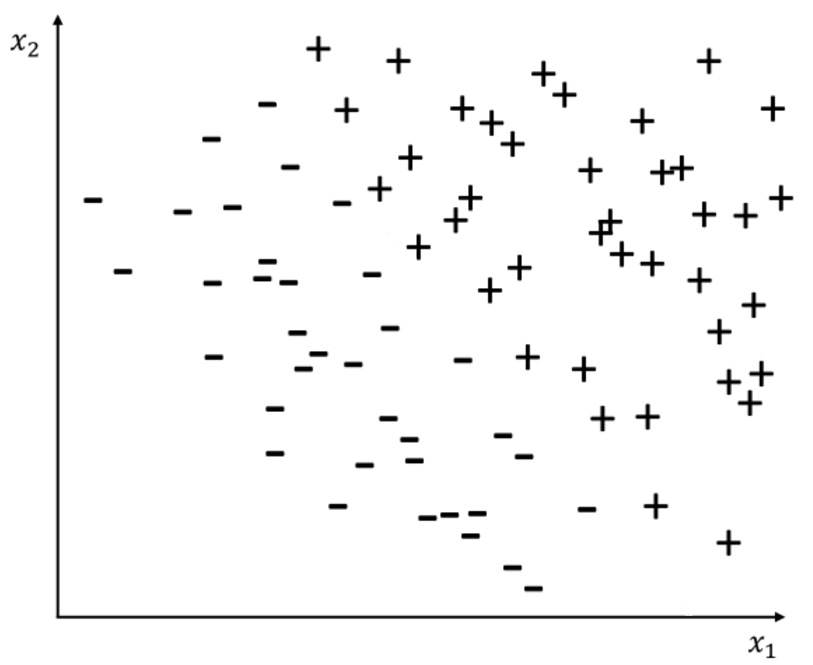
\includegraphics[width=\linewidth]{5a.png}
    \caption*{(5.1) Dataset}
  \end{subfigure}
  \begin{subfigure}[r]{0.3\linewidth}
    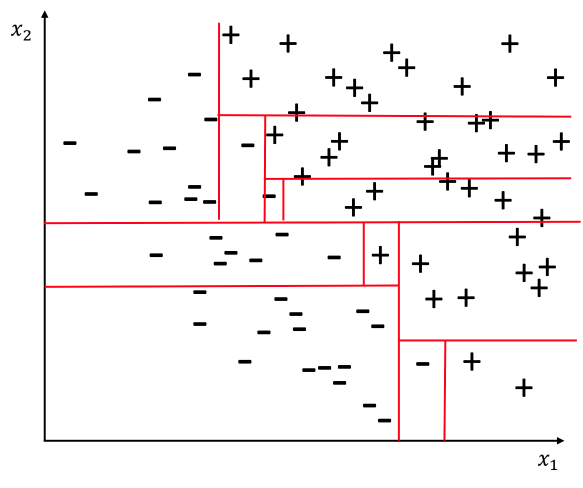
\includegraphics[width=\linewidth]{5b.png}
    \caption*{(5.2) Tree algorithm separating}
  \end{subfigure}
  \begin{subfigure}[r]{0.3\linewidth}
    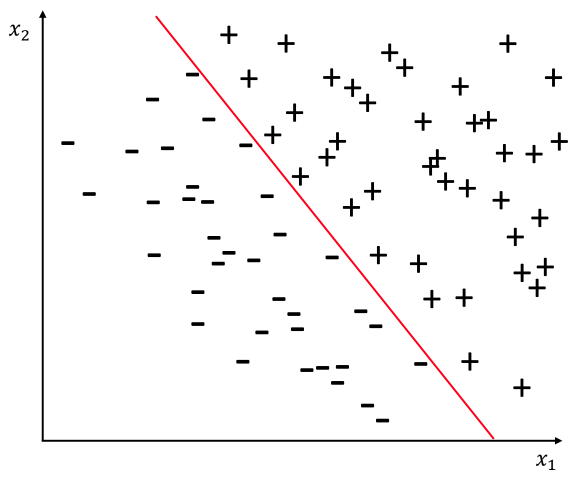
\includegraphics[width=\linewidth]{5c.png}
    \caption*{(5.3) Linear separating}
  \end{subfigure}
\end{figure}
}

\section{Linear Classifiers}

How do we separate? We define the hyperplane and the vector $w$ as the norm vector of that hyperplane and we multiply vector $x$ (from the dataset) by vector $w$. Then we find the threshold. If that\\ multiplication is over the threshold, we will say that $x$ in one class, and if it is under the threshold, $x$ will be in another class.
So this is a hypothesis [$h(x)$ возвращает $-1$ для класса Minus, $1$ для класса Plus]:
$$h(x)=sign\left(\langle w,x\rangle-threshold\right)$$
The one of the algorithms that utilise this hypothesis is called Perceptron.

\subsubsection*{Perceptron}

At the first step we should define a threshold and $w$. The vector $w$ is just a random vector. The threshold can be one of the coefficients of the vector $w$ (for example, $w_0$):
$$h(x)=sign\left(\langle w,x\rangle-w_0\right)$$
Then we can transform each vector $x$ of the dataset to simplify our $h(x)$ function: $$x=(x_1,\ldots,x_d)^T\to(1, x_1, \ldots, x_d)^T$$ After that transformation our hypothesis looks like that:
$$h(x)=sign\left(\langle w, x\rangle\right)=sign(w^Tx)$$
So we start with the random $w$ then we find such point $x$, when our hypothesis $h(x)$ does not match the answer $y$ (in case of two classes the hypothesis can be $1$ or $-1$). And then we just update $w$:
$$w_{new}=w_{old}+yx$$
[В конце концов после нескольких таких итераций мы остановимся. Гиперплоскость, перпендикулярная полученному вектору $w$ будет нашим ответом.]
Why would that work? Expalnation is quite simple: there is a theorem  that proves that it works in case of a linearly separable dataset. {\it <Some intuition about proof of this theorem>} And it actually works and works fast.

\subsubsection*{Pocket Algorithm}

If we have a linearly inseparable case, we have a Pocket Algorithm. {\it <An example with handwritten digits dataset>} A Pocket Algorithm is a simple modification of the Perceptron Algorithm: you just apply it for in given number of iterations and pick the best one in terms of validation dataset. It is called the Pocket Algorithm because you put your values in a pocket: when you find a new minimum you put it in the pocket and then you select the best partition from the pocket.

\subsubsection*{Feature Engineering}

The another way to fight a linearly inseparable dataset is adding new feature. For example [pic.~5.4] you can add feature like distance to (0,0) and get a linearly separable dataset [pic. 5.5].
\begin{figure}[h!]
  \centering
  \begin{subfigure}[l]{0.353\linewidth}
    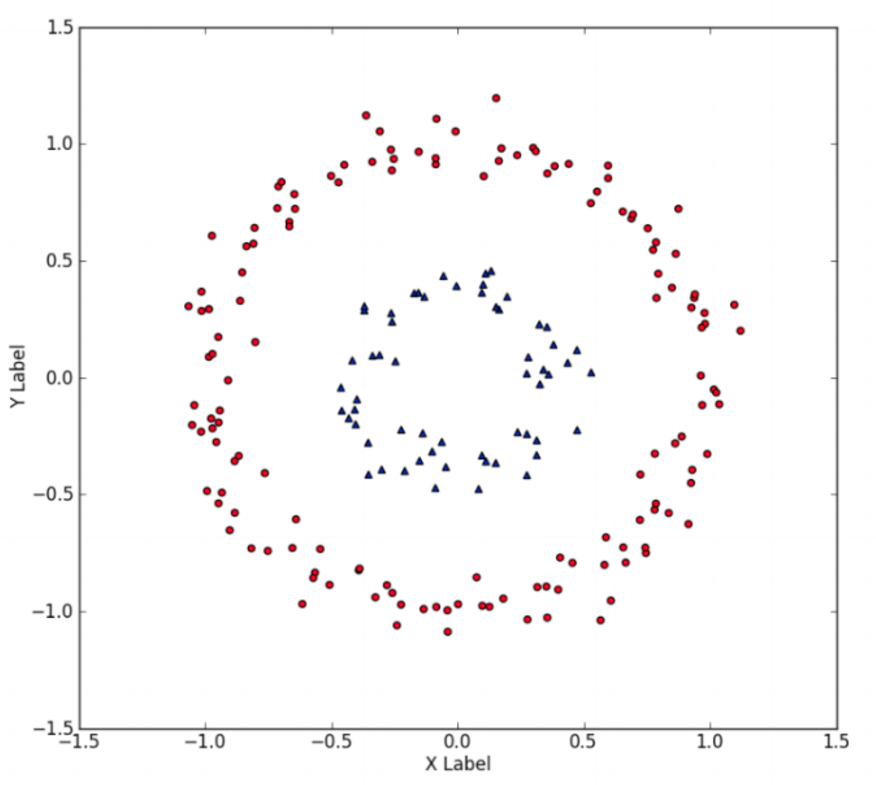
\includegraphics[width=\linewidth]{5d.png}
    \caption*{(5.4) Dataset in $\mathbb{R}^2$}
  \end{subfigure}
  \hspace{2cm}
  \begin{subfigure}[r]{0.4\linewidth}
    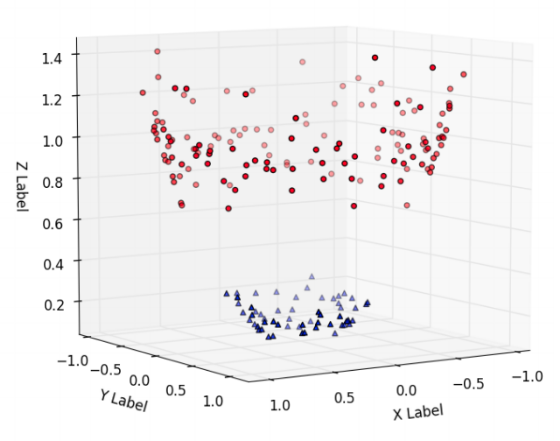
\includegraphics[width=\linewidth]{5e.png}
    \caption*{(5.5) Dataset in $\mathbb{R}^3$}
  \end{subfigure}
\end{figure}

\section{Theory of Error}

However, the problem is how many new features can we add. The more features we have the more overfitting we have.

\subsubsection*{Error in sample and error out of sample}

Let's say we have a dataset with $N$ points ($x_1,\ldots,x_N$), a general set $X$ [которое является абстрактым множеством данных, которые мы хотим классифицировать, например, все люди на Земле и т.д.] and an error function $err$ that somehow defines. An error in sample is
$$E_{in}(h)=\frac{1}{N}\sum\limits_{i=1}^N err(h(x_i),f(x_i))$$
And an error out of sample is
$$E_{out}(h)=E_X[err\left(h(x), f(x)\right)]$$
where $f(x)$ and $h(x)$ returns a class of a point $x$ ($f$ is the target function, $h$ is our hypothesis), $E_{out}$ is the mathematical expectation of our error function on a general set $X$. [$E_{err}$ мы никогда не можем подсчитать напрямую, только оценить. На практике это делается через validation и test датасеты.]\\

\subsubsection*{Hoeffding's inequality}

There is the Hoeffding's inequality:
$$P(|E_{in}(h)-E_{out}(h)|>\varepsilon)\le2e^{-\varepsilon^2N}$$
The difference $E_{in}(h)-E_{out}(h)$ is also called generalization error (sometimes in literature you can found $E_{out}$ as the generalization error). [The generalization error при заданном $h$ -- случайная величина в пространстве датасетов. Неравенство показывает, насколько хорошо ошибки гипотезы $h$ на датасетаx размера $N$ близки к ошибке $h$ на всем множестве $X$.] The big generalization error is a big overfitting and the small generalisation error is a small overfitting.\\
This inequality means for us that if we increase the dataset we exponentialy decrease the probability of overfitting for a one hypothesis. If we have a set of hypotheses then we have to multiply the right side by the $M$ -- number of hypotheses: 
$$P(|E_{in}(h)-E_{out}(h)|>\varepsilon)\le 2Me^{-\varepsilon^2N}$$
[В этом неравенстве $h$ -- лучшая из набора $M$ гипотез. Стоит отметить, что первое неравенство мы применять уже не можем: на разных датасетах лучшая из $M$ гипотез может быть разной.] If $M$ is small we can still guarantee mathematically that increasing the dataset does not get overfitting. Now the problem is how many hypotheses can we have. So this is a graph how our models behave ourselves in terms of complexity:
\begin{figure}[h!]
  \centering
  \begin{subfigure}[l]{0.7\linewidth}
    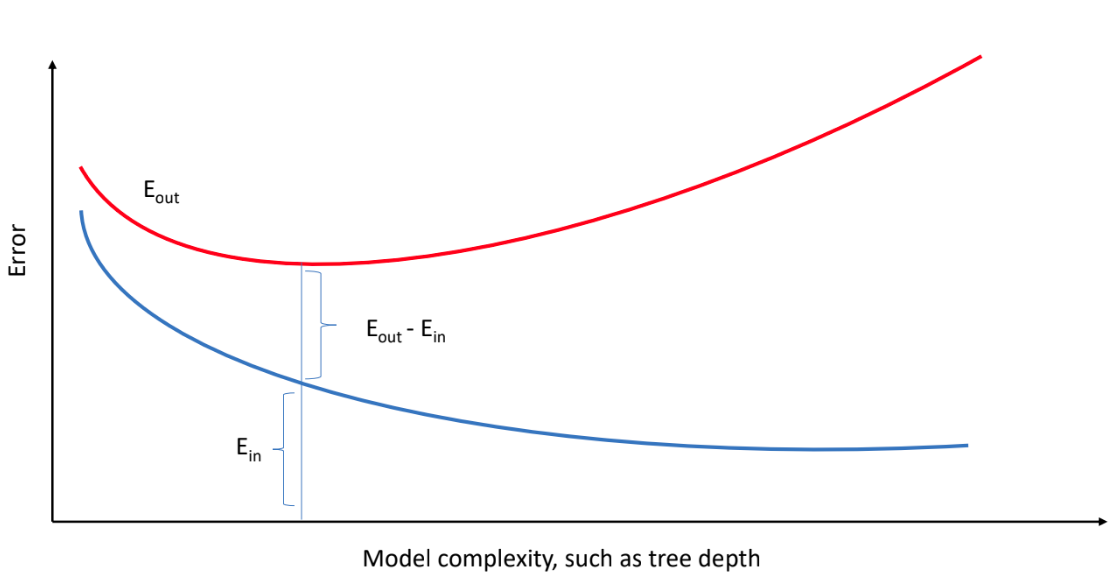
\includegraphics[width=\linewidth]{5f.png}
  \end{subfigure}
\end{figure}

\subsubsection*{From hypotheses to dichotomies}

Hovewer, even in a linear classification you don't have to go through all the hypotheses, for example, if you have some close hypotheses ($|E_{in}(h_1)-E_{out}(h_1)|\approx|E_{in}(h_2)-E_{out}(h_2)|$). So in terms of our math we'll go from hypotheses to dichotomies. The hypothesis is something that is defined for every point of the dataset and the dichotomy is also something that defined for every point of the dataset. But some dichotomies are not possible. [То есть некоторая гипотеза является дихотомией в зависимости от расположения точек из датасета относительно друг друга. К примеру, если вы используете для получения гипотез Perceptron Algorithm, то, чтобы некоторую гипотезу можно было назвать дихотомией, нужно чтобы в этой гипотезе классы были линейно отделимыми. В общем случае дихотомия типа H -- это гипотеза, которую можно получить алгоритмом H]. For example, if you set four points in four corners of the square, you will have only 14 dichotomies, because two dichotomies (where points in one edge have different class) you can not achive with Perceptron Algorithm. The actual number of the dichotomies is called the growth function:
$$m_H(N)=\max\limits_{x_1,\ldots,x_N}|H(x_1,\ldots,x_N)|$$
where $H(x_1,\ldots,x_N)$ is the set of possible dichotomies type $H$ on a points $x_1,\ldots,x_N$, $N$ is the number of points in the dataset. [Стоит понимать, что точки $x_i$ мы берем не из конкретного датасета. Мы берем все возможные расположения точек в пространстве (причем допускаются даже наложения точек друг на друга), считаем для каждого расположения количество возможных дихотомий, а затем берем макимум из подсчитанных значений.]

\subsubsection*{Vapnik-Chervonenkis inequality}

Now we can move from Hoeffding's inequality to Vapnik-Chervonenkis inequality:
$$P(|E_{in}(h)-E_{out}(h)|>\varepsilon)\le m_H(2N)\cdot4e^{-\varepsilon^{1/8}N}$$
The important thing that is now we have number of dichotomies that can be also exponential. And we still can't guarantee that in a big $N$ we will not overfit. However we can prove that the $m_H(2N)$ is almost always polynomial or less. How do we do that? 

\subsubsection*{Proof of polynomiality of a growth function in the presence of a breakpoint}

Well, the growth function is polynomial if it has what we called the breakpoint. The breakpoint is a $\min(k:m_H(k)<2^k)$ [Важно понимать, что для такого $k$ выполняется $\forall n\ge k\colon m_H(n)<2^n$]. In case of four points in 2D space, what we discussed already, $k=4$ is a breakpoint. <...> [Теперь перейдем к доказательству теоремы, используя новое понятие.\\
Пусть у нас есть набор из нескольких бинарных строк длины $N$, записанных в таблицу друг под другом ($i$-й столбец такой таблицы образован набором из $i$-тых символов всех строк). Известно, что для фиксированного $k$ выполнено следующее условие: если выбрать любые $k$ столбцов, то количество различных строк в выбранной части таблицы меньше $2^k$. Определим функцию $B(N,k)$ как наибольшее возможное количество строк в такой таблице.\\
Для начала покажем, что $\forall H\ B(N,k)\ge m_H(N)$, если breakpoint $m_H(N)$ равен $k$. Для этого убедимся, что все дихотомии типа $H$ длины $N$ можно вписать в таблицу с описанным правилом. Действительно, если у такой таблицы выбрать произвольные $k$ столбцов, то полученная таблица состоит из дихотомий длины $k$, значит, количество различных строк в выбранной части равно $m_H(N)<2^k$, что мы и хотели показать.\\
Теперь построим полиномиальную от $N$ оценку сверху на $B(N,k)$, тем самым получив ее и для $m_H(N)$. Для этого возьмем таблицу, удовлетворяющую описанным выше правилом, с наибольшим (т.е. равным $B(N,k)$) количеством строк. Разобьем строки этой таблицы на три части: $\alpha$, $\beta_+$ и $\beta_-$. Первая часть состоит из строк, у которых префикс длины $N-1$ уникален во всей таблице. Во вторую пойдут те из оставшихся, у которых последний символ равен $+1$, в третью, соответственно, $-1$. Таким образом $|\beta_+|=|\beta_-|=:b$. Обозначим $a:=|\alpha|$.\\
\begin{wraptable}{l}{5.8cm}
  \begin{tabular}{|c|c c c c|c|}
    \hline
    \multirow{5}{*}{$\alpha$} & +1 & +1 & $\ldots$ & +1 & +1 \\
                              & +1 & +1 & $\ldots$ & +1 & -1 \\
                              & $\vdots$ & $\vdots$ & $\vdots$ & $\vdots$ & $\vdots$ \\
                              & +1 & -1 & $\ldots$ & -1 & -1 \\
                              & -1 & +1 & $\ldots$ & -1 & +1 \\
    \hline
    \multirow{5}{*}{$\beta_+$}& +1 & -1 & $\ldots$ & +1 & +1 \\
                              & -1 & -1 & $\ldots$ & +1 & +1 \\
                              & $\vdots$ & $\vdots$ & $\vdots$ & $\vdots$& $\vdots$ \\
                              & +1 & -1 & $\ldots$ & +1 & +1 \\
                              & -1 & -1 & $\ldots$ & -1 & +1 \\
    \hline
    \multirow{5}{*}{$\beta_-$}& +1 & -1 & $\ldots$ & +1 & -1 \\
                              & -1 & -1 & $\ldots$ & +1 & -1 \\
                              & $\vdots$ & $\vdots$ & $\vdots$ & $\vdots$  & $\vdots$ \\
                              & +1 & -1 & $\ldots$ & +1 & -1 \\
                              & -1 & -1 & $\ldots$ & -1 & -1 \\
    \hline
  \end{tabular}
\end{wraptable}
Имеем следующее равенство:
$$B(N,k)=a+2b$$
Если мы возьмем префиксы длины $N-1$ строк из $\alpha\cup\beta_+$, то в полученной таблице любые $k$ столбцов образуют не более чем $2^k$ различных строк (поскольку таким свойством удовлетворяла исходная таблица). Значит:  
$$a+b\le B(N-1,k)$$
Теперь выберем префиксы длины $N-1$ строк из $\beta_-$. Заметим, что если в полученной таблице выбрать $k-1$ столбец, то различных строк в выбранной части будет меньше чем $2^{k-1}$ (иначе в исходной таблице столбцы с теми же номерами вместе с $N$-тым содержали бы не менее $2^{k-1}$ различных строк из $\beta_-$ и столько же соответствующих им строк из $\beta_+$, что в сумме дает $2^k$ различных строк, а это невозможно в исходной таблице по построению). Тем самым мы получили:
$$b\le B(N-1,k-1)$$
Суммируя последние два выражения, получаем:
$$B(N,k)=\alpha+2\beta\le B(N-1, k)+B(N-1,k-1)$$
Теперь мы можем показать следующую оценку:
$$B(N,k)\le\sum\limits_{i=0}^{k-1}\binom{N}{i}$$
Знаем, что $B(N,1)=1$, $B(1,k>1)=2$ и $\binom{N-1}{i-1}+\binom{N-1}{i}=\binom{N}{i}$, значит, использую индукцию по $N$ и $k$, можем показать:
$$B(N,k)\le B(N-1,k)+B(N-1,k-1)\le\sum\limits_{i=0}^{k-1}\binom{N-1}{i}+\sum\limits_{i=0}^{k-2}\binom{N-1}{i}=$$ $$=1+\sum\limits_{i=1}^{k-1}\binom{N-1}{i}+\sum\limits_{i=1}^{k-1}\binom{N-1}{i-1}=1+\sum\limits_{i=1}^{k-1}\binom{N}{i}=\sum\limits_{i=0}^{k-1}\binom{N}{i}$$
Последняя сумма является многочленом от $N$.]

\subsubsection*{VC-dimention}

$d_{VC}(H)$ for hypotheses type $H$ is the maximum number $N$ such that $m_H(N)=2^N$. If $k$ is the breakpoint, $d_{VC}=k-1$, so:
$$m_H(N)=B(N,k)\le\sum\limits_{i=0}^{k-1}\binom{N}{i}=\sum\limits_{i=0}^{d_{VC}}\le N^{d_{VC}}+1$$
Why is this important? Because we can pull that in the Vapnik-Chervonenkis inequality and guarantee that we don't overfit in a big dataset. And the number $d_{VC}$ shows the effective complexity of a model.

\subsubsection*{VC-dimention for perceptron}

Now we prove that if $d$ is the space dimensionality, $d_{VC}=d+1$ [для случая, когда классы в дихотомии линейно разделимы].\\
So we have $d$ dimentions and at first we prove that we can have all the posible dichotomies for $d+1$ points. Let's construct the set of these points [не забываем добавить $d+1$'ую размерность, координата которой у всех точек из датасета равна 1]:
$$X=
\begin{pmatrix}
  x_1^T \\
  x_2^T \\
  x_3^T \\
  \ldots \\
  x_{d+1}^T
\end{pmatrix}
=
\begin{pmatrix}
  1 & 0 & 0 & 0 & \ldots & 0 \\
  1 & 1 & 0 & 0 & \ldots & 0 \\
  1 & 0 & 1 & 0 & \ldots & 0 \\
    &   &   & \vdots \\
  1 & 0 & 0 & 0 & \ldots & 1
\end{pmatrix}
$$
And we get invertable matrix, so we can solve this [обозначения как в описании Perceptron Algorithm: $y$ -- классы точек, $w$ -- нормаль к гиперплоскости, которую мы ищем]:
$$sign(Xw)=y;$$
$$Xw=y;$$
$$w=X^{-1}y.$$
Now we only need to prove that we can't have all hypotheses as dichotomies in $d+2$ points. So let's take $x_1,\ldots,x_{d+1},x_{d+2}$.  If two points from them are the same we already can't have all dichotomies. If there's not same points, let's assume that all hypotheses on that points are dichotomies. Because we work in $d+1$ dimentional space [$d+1$'ая размерность -- та, которая состоит из едениц] there is a vector $x_j$ that can be expressed to a linear combination of other $d+1$ vectors:
$$x_j=\sum\limits_{i\ne j}a_ix_i;$$
$$y_j=sign(w^Tx_j)=sign\left(\sum\limits_{i\ne j}a_iw^Tx_i\right).$$
If $y_i=sign(a_i)$ the $y_j$ can't be $-1$ (because $\forall i\ne j\ a_iw^Tx_i$ is always positive [так как $a_i$ и $w^Tx_i$ одного знака, поскольку мы так определили $y_i$]), so our assumption is incorrect and we prove the theorem.

\subsubsection*{Sufficient data}

So we proved that for perecptron algorithm:

$$P(|E_{in}(h)-E_{out}(h)|>\varepsilon)\le m_H(2N)\cdot4e^{-\varepsilon^{1/8}N}\approx N^{d_{VC}}e^{-N}$$

What does that give us? Well, if you want a nice hypothesis and if you don't want overfit you'd better have sufficient data: when $N\ge 10d_{VC}$ everything is OK. The problem is how to get the $d_{VC}$. For perceptron we have already get, for neural network we can calculate $d_{VC}$ as well because we can find the breakpoint. And what we do in the real world is the validation.

\section{Validation}

[Валидация -- процесс подбора оптимальных параметров обучающего алгоритма, используя заранее подготовленную для этого выборку. В отличие от валидации, тестирование и тестирующая выборка из датасета нужны для сравнения работы разных алгоритмов.]\\
Why is validation work? It works because dichotomy inequality works in it's original form, because we train our hypotheses on our dataset. So the validation is just pass the best hypothesis. There is an inequality for one hypothesis:
$$P(|E_{val}(h)-E_{out}(h)|>\varepsilon)\le2e^{-\varepsilon^2N}$$
Now the problem is: if you have many various parameters and so on then if you start pasting many hypotheses to your validation dataset you have to multiply right side by the number of hypotheses. That is why we go from validation to testing. That is why we train, validate and test. Because of Hoeffding's inequality. So you train on train dataset then you pass your answer on your validation dataset and you estimate the overfitting. The proper validation size is $K=\frac{N}{5}$ ($N$ is number of points in your dataset).

\subsubsection*{Cross-validation}

The problem with validation is we don't use all points. The validation dataset has only $20\%$ of all points and we don't use that points in our training. That is bad, because points are usualy expensive: you spend money for each point you have. So we do want to use them all. The thing what helps us is caled cross-validation.\\
The cross validation is the way to use all the points. We separate all dataset on 10 datasets, and take one of them as a validation dataset and all the others as a training dataset. And repeat. Now we should talk about data leaking.

\subsubsection*{Data leaking}

%Let's imagine you have a EEG signal from five pacients and you need to predict an epileptic seizure. The signals looks like this:\\
%{\it <One day there will be a pic>}\\
%And at some points in the EEG you have an epileptic seizures. You can say: Ok, let's have the validation dataset, let's have a trainig dataset. But you can divide your EEG diagrams like this:\\
%{\it <One day there will be a pic>}\\
%<...> What polutes your dataset. So you should divide like this:\\
%{\it <One day there will be a pic>}\\
{\it <Examples with EEG and MRT>}

\subsubsection*{Train $\rightarrow$ Validate $\rightarrow$ Test}

\begin{enumerate}[label=$\bullet$]
  \item Train the algorithm on your train dataset.
  \item Optimize hyperparameters on validation (or crossvalidation).
  \item Check the final perfomance on test.
\end{enumerate}

\chapter{Neural Networks}

{\sf An inspiration to a neural networks mashines comes from biological neural networks. In 1950's we already knew how it works. The the main thing that allows a neuron to filter all the useless signals that happend in the brain all the time is all-or-none law: if a signal exceeds the threshold potential, the neuron will give a complete response; otherwise, there is no response.}

\section{Perceptron}

So the perceptron works the same. However, it can be represented as the small neural network where input neurons are the signals what multiplied by some coefficients, then all results add up and if sum is over some threshold, we get the signal $+1$, otherwise, we get $-1$. The problem with that is we can only have one layer: if you combine several layers as how it happens in the brain, you will have no good way of training the multi-layer perceptron with the simple threshold function. So the way around it is replace the threshold function for something more complex. The first aproach is a single layer neural network with logistic function as a threshold.

\section{Single Layer Networks}

The single layer neural network with logistic function is called logistic regression. The logistic regression is the classification algorithm, not the regression algorithm. It's just called like that.

\subsubsection*{Logistic regression}

For the binary classification (with classes $+1$ and $-1$) the math comes out very nicely; the probability of the signal is the one minus the probability of the reverse signal:
$$P(y|x)=\begin{cases}
f(x)&\text{for }y=+1,\\
1-f(x)&\text{for }y=-1.
\end{cases}$$
This sigmoid function $\sigma$ satisfies the both parameters of $P(x|y)$:
$$P(y|x)=\sigma(yw^Tx),\qquad\sigma(s)=\frac{1}{1+e^{-s}},\qquad \sigma(s)=1-\sigma(s)$$
where $w^Tx$ is the answer of the perceptron in input $x$.\\
So if our output is the probability of classes, how would we calculate the loss function? How we would calculate the error what we can try to minimize? Well, we just use likelyhood:
$$\prod\limits_{i=1}^{N}P(y_i|x_i)=\prod\limits_{i=1}^{N}\sigma(y_iw^Tx_i)$$
Then we go from multiplication to sum of the logarithms and get loss function (what we will try to minimize) for the logistic regression:
$$L(w)=-\frac{1}{N}\ln\left(\prod\limits_{i=1}^N\sigma(y_iw^Tx_i)\right)=\frac{1}{N}\sum\limits_{i=1}^N\ln(1+e^{-y_iw^Tx_i})$$

Now the problem is training it. Even for one layer logistic regression we need to utilise the gradient descent:
$$w(t+1)=w(t)-\eta\frac{\partial C(w)}{\partial w}$$
The $C(w)$ is the cost function (instead it we can the use loss function; we typically talk about the loss function $L(w)$ (or $J(w)$) and the cost function $C(w)$). And we have the learning rate $\eta$.\\
In case of large data it becomes hard to calculate the average value of all logarithms in the loss function $L(w)$. However, we can go around by using a stochastic gradient descent: just calculate the loss function for batch (some part of the data) and then apply the gradient descent step for that batch. So if we use the stochastic gradient descent, at first we need to split our data into random batches and complete the gradient descent step for every batch. This iteration is called an epoch. The number of steps in one epoch is number of all points divided by the size of the betch ($N / N_{batch}$).
So this is the difference beteen the gradient descent and stochastic gradient descent:
$$\text{Gradient Descent: }w\leftarrow w-\eta\left(-\frac{1}{N}\sum\limits_{i=1}^N\frac{y_ix_i}{1+e^{y_iw^Tx_i}}\right)$$
$$\text{Stochastic Gradient Descent: }w\leftarrow w-\eta\left(-\frac{1}{N_{batch}}\sum\limits_{x_i\in batch}\frac{y_ix_i}{1+e^{y_iw^Tx_i}}\right)$$
Also we have a very stochastic gradient descent (when every bench contains only one point).\\
%$$w\leftarrow w-\eta\frac{\partial C(w^Tx_i,y_i)}{\partial w}$$
{\it <The reason why very stochastic gradient descent is not the best way>}

\section{Several Layers Networks}

So we have the algorithm for training in one layer neural network. The way to trainig the several layers is the back-propagation. 

\subsubsection*{Back-propagation}

At first we need to define some coefficients and numbers:
\begin{enumerate}[label=$\bullet$]
  \item $w_{jk}^l$ is the weight between neuron $j$ in layer $l-1$ and neuron $k$ in layer $l$.
  \item $x_j^l$ is the outcoming signal after the activation function, i.e. $x_j^l=\sigma\left(\sum w_{ij}^lx_i^{l-1}\right)$ (for the logistic regression $\sigma$ is the sigmoid function). In the first layer $x_j^1=x_j$ ($x_j$ is a feature). You can look at all $x_i^l$ in other layers at the features as well (sometimes they called feature layers).
  \item $s_j^l$ is the incoming signal to neuron $j$ in layer $l$, $s_j^l=\sum w_{ij}^lx_i^{l-1}$
\end{enumerate}
So the values what we try to optimise is $w$'s. We want to calculate the gradient for loss functions over the $w$'s. This is the goldest way to calculate the partial derilivative of our loss function:
$$\nabla C_{w_{ij}^l}(w)=\frac{\partial C(w)}{\partial w_{ij}^l}=\frac{\partial C(w)}{\partial s_j^l}\times\frac{\partial s_j^l}{\partial w_{ij}^l}$$
Also we have
$$\frac{\partial s_j^l}{\partial w_{ij}^l}=x_i^{l-1}$$
because $s_j^l=\sum w_{ij}^lx_i^{l-1}$. Then we calculate $\delta_j^{l-1}$ what is defined as
$$\delta_j^{l-1}=\frac{\partial C(w)}{\partial s_j^{l-1}}$$
If the loss function $f$ is diferantionable then we just calculate all partial derilivatives for the last layer $L$:
$$\delta_i^L=\frac{\partial C(w)}{\partial s_i^L},\qquad C(w)=f(x^L),\qquad x_i^L=\sigma(s_i^L)$$
For the previous layers we can again apply the chain rule and calculate the $\delta_i^{l-1}$ using $\delta_i^l$:
$$\delta_i^{l-1}=\frac{\partial C(w)}{\partial s_i^{l-1}}=\sum\limits_{j}\frac{\partial C(w)}{\partial s_j^l}\times\frac{\partial s_j^l}{\partial x_i^{l-1}}\times\frac{\partial x_i^{l-1}}{\partial s_i^{l-1}}=\sum\limits_{j}\delta_j^l\times w_{ij}^l\times\sigma'(s_i^{l-1})$$
So back-propagation algorithm looks like this:
\begin{enumerate}[label=\arabic*.]
  \item Initialize weights randomly (with small random numbers in $[-0.1,0.1]$).
  \item Compute the forward path: calculate all $x$ and $s$.
  \item Go backward and calculate all $\delta$.
  \item Shift all weights: $w_{ij}^l\leftarrow w_{ij}^l-\eta x_i^{l-1}\delta_j^l$ ($\eta$ is some learning rate).
  \item Go to step 2.
\end{enumerate}
The important thing is you can calclulate all $\delta$ with tensors: you don't have to iterate over each coefficient but rather multiply tensors. Which is good because we can push it into the GPU's what are really good in multiplying thensors.

\subsubsection*{Activation functions}

Sigmoid: 
$$\sigma(s)=\frac{1}{1+e^{-s}}$$
Tanh:
$$\sigma(s)=\frac{e^s-e^{-s}}{e^s+e^{-s}}$$
Rectified Linear Unit (ReLU):
$$\sigma(s)=\max(0,s)$$
The sigmoid finction goes from 0 to 1. If you want something what can be negative you can use hyperbolic tangent what goes from $-1$ to 1. And if you want something what calculates very fast and doesn't get your gradient diminished when you reach big numbers you can use ReLU.

\subsubsection*{Softmax and cross-entropy}

In case of binary classification you use logistic function and you have one output neuron what gets the probability of one class. In multiclass classification case we utilize the function what is called the Softmax:
$$x_j^L=\sigma^L(s_j^L)=\frac{e^{s_j^L}}{\sum e^{s_i^L}}$$
It is called Softmax because all last layer neurons output numbers around 0 (exept one that outputs number around 1).\\
The cross-entropy loss function is:
$$C(w)=\sum o_i\log(x_i^L),\qquad o_i=\begin{cases}
1&\text{if }y=i,\\
0&\text{if }y\ne i.
\end{cases}$$
{<\it Some talk what I can't understand>}\\
The networks what are orginised like that is called fully conected network: each neuron of the one layer connects with each neuron of the next layer and so on.

\section{Regularization}

Networks, espesualy fully conected, are very prompt to overfitting. For example let's say we have a very big network and train it to recognize images. Instead of learning features of the images, for example, recognizing a cat from a car by ears and so on, big neural networks can just memorize the images: it can looks on the value of concrete pixel. This is an overfitting -- memorising the dataset,  noise training and so on. How we can to regularize it? 

\subsubsection*{L2 regularization}

When we regularize we trying to lower the VC-dimention, lower the number of possible hypotheses. We do that by adding some constraints to the loss function. Here we add the L2 constraint:
$$C_{new}(w)=C(w)+\frac{\lambda}{2N}\|w\|_2^2$$
This way is called the L2 regularization or weight decay.\\
{\it <Some intuition why it works>} %If you look at the derilivative of the funсtion $C_{new}$ you will have derilivative of the loss function $C(w)$ and the negative weight. <...>

\subsubsection*{Early stopping}

The another way in regularization is catching the moment of overfitting. So this is a typical graph what shows gain between errors on the validation dataset and training dataset (the x axis is the number of epochs):\\
{\it <Pic>}\\
The error on the training dataset is always decrease, but error in the validation dataset in some point starts to increase. And at that point we want to stop (remember the weights of the network in that point).

\subsubsection*{Dropout}

Dropout is a direct way to preventing networks from memorizing the dataset. We just turn of some (50\%, for example) random neurons for every layers in every patch. The turned of neuron outputs 0. In that way the network will try to learn general features rather than specific pathways, because each pathway can be turned off.\\
When we apply this network at some task we need to turn on all the neurons.

\subsubsection*{Data augmentation}

The overfitting doesn't happen if you have a lot of data. How to create a lot of data we will talk at the next lecture.

\section{Deep Learning Libraries}

If you don't like Python, learn to like Python because most of deep learning done in it. However there is still some inthusiasts what work on the deep learning for Java \href{http://deeplearning4j.org/}{library}.\\
Google represents \href{www.tensorflow.org}{TensorFlow} and the \href{keras.io}{Keras} (what is built on top of the first one). So if you just want to create networks simply you should use Keras. And if you want to create complex networks you should use TensorFlow.\\
The \href{torch.ch}{Torch} library easier than TensorFlow but more complex than Keras.

\end{document}